\documentclass[IB]{PlantillaPACnova_Est}
\usepackage{hyperref} %url amb \ref. 
\usepackage{float}
\usepackage{amsmath}
\usepackage{hyperref}
\usepackage{pgfplots}
\usepackage{xcolor}
\usepackage{tikz}
\usepackage{url}
\usepackage{wrapfig}
\usepackage{natbib}
\usepackage{geometry}
\usepackage{graphicx}
\usepackage{tikz-er2}
\usepackage{ragged2e}
\usepackage{caption}
\usepackage[section]{placeins}
\def\vi{\vec{\i} }
\def\vj{\vec{\j} }
\def\vk{\vec{k} }
\def\vk{\vec{k} }
\def\vB{\vec{B} }
\def\vH{\vec{H} }
\def\vM{\vec{M} }
\def\vE{\vec{E} }
%\def<d{/>{\rm d}}
\def\vr{\vec{r}}
\def\Ohm{\Omega}
\def\qpi{\frac{1}{4\pi\varepsilon_0}}
\DeclareMathSymbol{,}{\mathord}{letters}{"3B}
%\usepackage{siunitx}
%\DeclareSIUnit\grau{\degreeCelsius}
%\sisetup{output-decimal-marker = {,}}
%\sisetup{per-mode = symbol}%
%\sisetup{exponent-product = \cdot}
%\usepackage{upgreek}
%\usepackage{cancel}
\setcounter{secnumdepth}{0} 
\usepackage[nottoc,numbib]{tocbibind}
\usepackage{tocloft}
\renewcommand{\cftsecleader}{\cftdotfill{\cftdotsep}}
\bibliography{biblio.bib} 
% Colores de las barras
\definecolor{bblue}{HTML}{4F81BD}
\definecolor{rred}{HTML}{C0504D}
\definecolor{ggreen}{HTML}{9BBB59}
\definecolor{ppurple}{HTML}{9F4C7C}
\captionsetup{justification=centerlast,labelfont=bf,textfont=it}

\begin{document}
\textinicial
%%%%%%%%%%%%%%%%%%%%%%%%% Código %%%%%%%%%%%%%%%%%%%%%%%%%%%%%%%% --------------------> 1
{M2.851} 				
%%%%%%%%%%%%%%%%%%%%%%%%% Assignatura %%%%%%%%%%%%%%%%%%%%%%%%%%--------------------> 2
{Tipología y ciclo de vida de los datos}
%%%%%%%%%%%%%%%%%%%%%%%%% Número de PEC o Práctica %%%%%%%%%%%%%--------------------> 3
{PRA1}
%%%%%%%%%%%%%%%%%%%%%%%%% Curso i número de semestre %%%%%%%%%%%%--------------------> 4
{2021-22-Sem.2}
%%%%%%%%%%%%%%%%%%%%%%%%% Nombre Programa %%%%%%%%%%%%%%%%%%%%%%%%%--------------------> 5
{Master de ciencia de datos}
%%%%%%%%%%%%%%%%%%%%%%%%% Vuestro nombre %%%%%%%%%%%%%%%%%%%%%%%%%--------------------> 6
{Maria Dolores Moyano Guerrero y Víctor Cáncer Castillo}




\begin{center}
\textbf{{\LARGE PRA 1 - Tipología y ciclo de vida de los datos}}\\[1cm]

\textbf{{\Large Maria Dolores Moyano Guerrero y Víctor Cáncer Castillo}}
\end{center}

\tableofcontents
\newpage 

\section{Contexto}
\paragraph{Explicar en qué contexto se ha recolectado la información. Explicar por qué el sitio web elegido proporciona dicha información.\\} 
Estos datos se han recogido para practicar el \textit{web scraping} en la asignatura de \textit{Tipología y ciclo de vida de los datos} del Máster de ciencia de datos de la UOC.\\
Cómo (futuros) científicos de datos hemos tenido la curiosidad de estudiar cómo está el mercado laboral actualmente en varias ciudades europeas y americanas. Además hemos querido averiguar en qué lugares el trabajo de científico de datos está más reconocido por las empresas y por lo tanto mejor remunerados. \\
Para ello hemos obtenido los sueldos que se ofrecen por diferentes empresas utilizando la web \textit{\url{https://glassdoor.es/}}, donde los trabajadores pueden informar de su sueldo de manera anónima. Por otro lado hemos extraído datos de la web \textit{ \url{https://datosmacro.expansion.com/}} dónde hay múltiples datos económicos, entre ellos el salario medio, lo cual nos puede mostrar si el trabajo del científico de datos está mejor/peor remunerado que el resto de trabajos en ese pais o ciudad.

\begin{figure}[h]
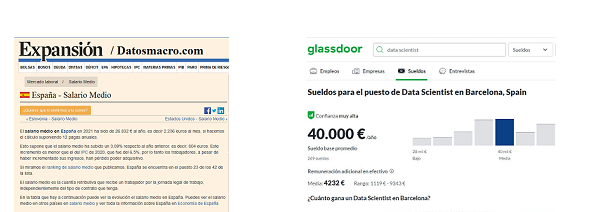
\includegraphics{fuentes.png}
\caption{Captura de las páginas webs utilizadas para el estudio}
\end{figure}

\newpage 
\section{Título}
\paragraph{Definir un título que sea descriptivo para el dataset.\\}

El título que describe el dataset final es: comparación de los sueldos para un científico de datos en determinadas ciudades con el sueldo medio de los países donde radican dichas ciudades.

\section{Descripción del dataset}
\paragraph{Desarrollar una descripción breve del conjunto de datos que se ha extraído. Es necesario que esta descripción tenga sentido con el título elegido.\\}

Para las ciudades descritas se recogen los datos:
\begin{itemize}
\item \textit{Sueldos\_DataScientist\_vs\_SMI}: Comparación de los sueldos de las distintas ciudades con el Sueldo Medio.
\item \textit{SMI.csv}: Contiene los sueldos medios de un listado de países.
\item \textit{dataset\_sueldos.csv}: Sueldos extraídos para científicos de datos en distintos periodos.
\item \textit{dataset\_sueldos\_clean.csv}: Sueldos de un científico de datos para un año.
\end{itemize}

\newpage
Los datos obtenidos recogen los datos siguientes:
\\
\begin{figure}[h]
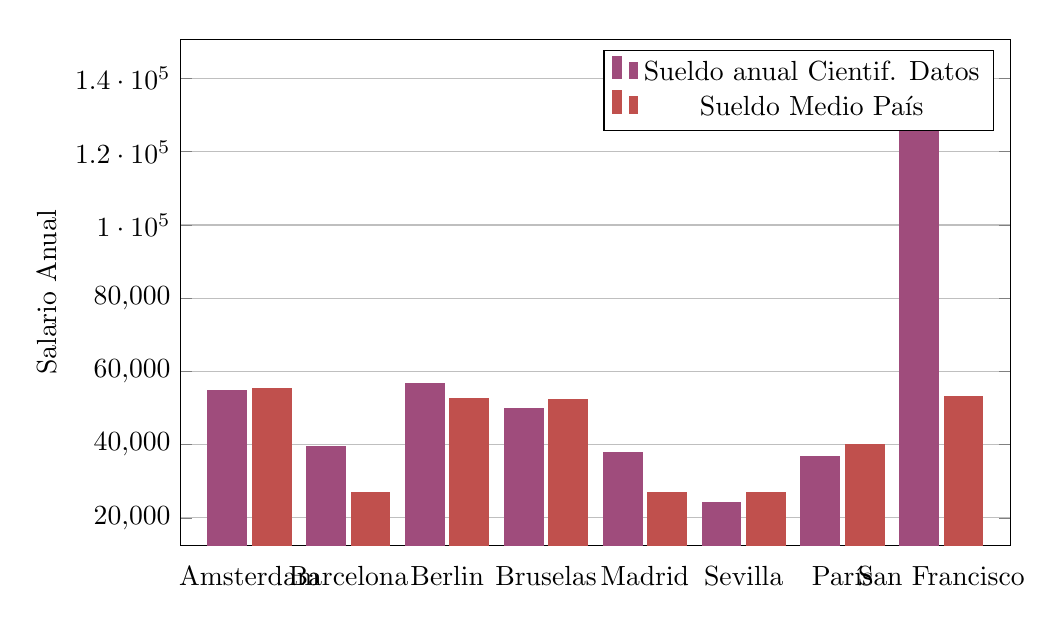
\begin{tikzpicture}
    \begin{axis}[
        width  = 1*\textwidth,
        height =8cm,
        major x tick style = transparent,
        ybar,
        bar width=14pt,
        ymajorgrids = true,
        ylabel = {Salario Anual},
        symbolic x coords={Amsterdam,Barcelona,Berlin,Bruselas,Madrid,Sevilla, París,San Francisco},
        xtick = data,
        scaled y ticks = false,
    ]
        \addplot[style={ppurple,fill=ppurple,mark=none}]
        coordinates {(Amsterdam,54806.39) (Barcelona,39446.56) (Berlin,56582.98) (Bruselas,49850.48) (Madrid,37893.96)(Sevilla,24073.81) (París,36858.89)(San Francisco,139090.03)};
            
         \addplot[style={rred,fill=rred,mark=none}]
        coordinates {(Amsterdam,55338.99) (Barcelona,26832.00) (Berlin,52556.02) (Bruselas,52248.02) (Madrid,26832.00)(Sevilla,26832.00) (París,39970.99)(San Francisco,53229.00)};

      
        \legend{Sueldo anual Cientif. Datos,Sueldo Medio País}
    \end{axis}
\end{tikzpicture}
\caption{Comparación de los sueldos de científico de datos en las ciudades estudiadas}
\end{figure}
\newpage 

\section{Representación gráfica}
\FloatBarrier
\paragraph{\\Dibujar un esquema o diagrama que identifique el dataset visualmente y el proyecto elegido.\\}
\FloatBarrier
\begin{figure}[h]
\usetikzlibrary{positioning}
\usetikzlibrary{shadows}

\tikzstyle{every entity} = [top color=white, bottom color=blue!30, 
                            draw=blue!50!black!100, drop shadow]
\tikzstyle{every weak entity} = [drop shadow={shadow xshift=.7ex, 
                                 shadow yshift=-.7ex}]
\tikzstyle{every attribute} = [top color=white, bottom color=yellow!20, 
                               draw=yellow, node distance=1cm, drop shadow]
\tikzstyle{every relationship} = [top color=white, bottom color=red!20, 
                                  draw=red!50!black!100, drop shadow]
\tikzstyle{every isa} = [top color=white, bottom color=green!20, 
                         draw=green!50!black!100, drop shadow]
\centering
\scalebox{.87}{
\begin{tikzpicture}[node distance=1.5cm, every edge/.style={link}]

  \node[entity] (pai) {Pais};
  \node[attribute] (smi) [above=of pai] {SueldoMedio} edge (pai);
  \node[attribute] (anio) [right=of pai] {Anio} edge (pai);
  \node[attribute] (mon) [below right=of pai] {Moneda} edge (pai);
  \node[attribute] (nom) [above right=of pai] {Nombre} edge (pai);

  \node[relationship] (pertenece) [left=of pai] {Tributa} edge (pai);

  \node[entity] (emp) [below=of pertenece] {Empresa} edge (pertenece);
  \node[attribute] (nombe) [left=of emp] {Nombre} edge (emp);  

  \node[relationship] (ofrece) [below=of emp] {Oferta  } edge  (emp);

  \node[entity] (Pue) [right=of ofrece] {Puesto} edge (ofrece);
  \node[attribute] (per) [below=of Pue] {Periodo} edge (Pue);
  \node[attribute] (suele) [right=of Pue] {Sueldo} edge (Pue);  
  \node[attribute] (nombp) [below right=of Pue] {Nombre} edge (Pue);  
  
  \node[relationship] (esta) [below=of pai] {Está en} edge  (Pue);
  \draw[link] (Pue.27) -| (esta) (esta) edge (pai);

\end{tikzpicture}
}
\caption{Diagrama de las entidades principales del proyecto}
\end{figure}
\FloatBarrier

\newpage 
\section{Contenido}
\paragraph{Explicar los campos que incluye el dataset, el periodo de tiempo de los datos y cómo se han recogido.\\}
Dataset\_sueldos.csv: se ha obtenido de la página  \textit{\url{https://glassdoor.es/}} el 6/4/2022. No ha sido necesario recoger los datos en varios días debido a la naturaleza del proyecto.
\begin{itemize}
\item \textbf{Ciudad:} Ciudad donde está radicado el empleo.
\item \textbf{Empresa:} Empresa que proporciona el empleo.
\item \textbf{Sueldo:} Sueldo bruto correspondiente al empleo, ciudad y empresa.
\item \textbf{Periodo:} Empleo en el periodo indicado, en su caso.
\end{itemize}

Dataset\_sueldos\_clean.csv: se ha obtenido de la página  \textit{\url{https://glassdoor.es/}} el 6/4/2022. No ha sido necesario recoger los datos en varios días debido a la naturaleza del proyecto.
\begin{itemize}
\item \textbf{Ciudad: } Ciudad donde está el empleo.
\item \textbf{Empresa:} Empresa que proporciona el empleo.
\item \textbf{Sueldo:} Sueldo bruto correspondiente al empleo, ciudad y empresa.
\item \textbf{Sueldo Anual:}. Sueldo ajustado a un año (algunas empresas, no lo proporcionan anualizado).
\end{itemize}

SMI.csv: se ha obtenido de la página  \textit{\url{https://datosmacro.expansion.com/}} el 6/4/2022. No ha sido necesario recoger los datos en varios días debido a la naturaleza del proyecto.
\begin{itemize}
\item \textbf{País: }País que se corresponde al sueldo medio.
\item \textbf{Año: }Año de cálculo del sueldo medio.
\item \textbf{SalMed Local: }Salario medio en moneda local.
\item \textbf{Moneda:} Moneda del salario local.
\item \textbf{Salmed \$:} Salario medio en dólares.
\item \textbf{Salmed €:} Salario medio en euros.
\item \textbf{Var:} Variación del salario medio.
\end{itemize}
\newpage
Sueldos\_DataScientist\_vs\_SMI: Se han calculado a partir de los datos extraidos en las páginas descritas.
\begin{itemize}
\item \textbf{Ciudad:}  Ciudad donde está el empleo.
\item \textbf{Sueldo anual:} Sueldo anual de los empleos descargados.
\item \textbf{Suelvo vs Sueldo Medio: }Diferencia entre el sueldo del puesto de Científico de Datos y el sueldo medio del país.
\end{itemize}

\section{Agradecimientos}

Agradecemos a los propietarios de las páginas  \textit{\url{https://glassdoor.es/}} y \textit{ \url{https://datosmacro.expansion.com/}}, por los datos de los que nos hemos podido alimentar en este proyecto de Web Scraping. 

\section{Inspiración}

En el actual contexto, donde las comunicaciones permiten buscar trabajo en distintos destinos sin tener que desplazarse, y además es posible trabajar en remoto, los sitios webs que permiten buscar trabajo y comparar sueldos son una herramienta muy útil a la hora de escoger el puesto más conveniente. Los datos recogidos son interesantes porque permiten comparar los sueldos de los científicos de datos en caliente, utilizando el factor de corrección del sueldo medio del país, para poder analizar si efectivamente esos puestos de trabajo son valorados en la ciudad donde se demandan y así tener un mapa claro de la situación, para prestar ayuda a los demandantes de empleo de esta disciplina. 

Este proyecto podría ampliarse a la búsqueda de trabajo para otra tipología de puestos, simplemente, modificando la búsqueda.

\newpage 
\section{Licencia}
Se ha escogido la licencia CC BY-SA 4.0 ya que es la más correcta en cuanto a las libertades que se han de cumplir:
\\
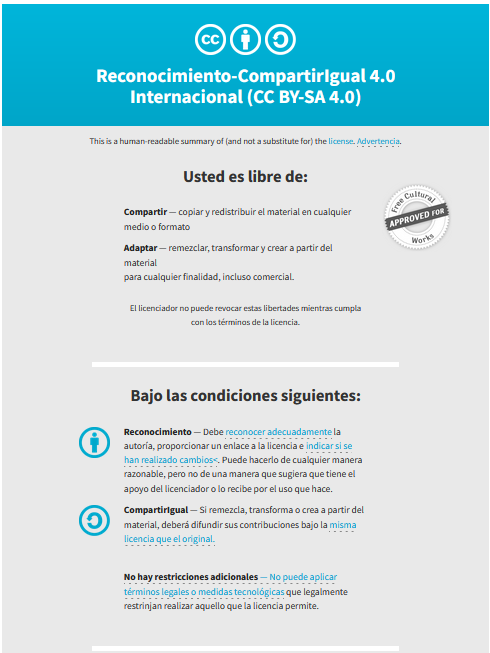
\includegraphics [scale=0.75]{licencia1.png}
\\

\includegraphics [scale=0.75]{licencia2.png}


\section{Código}

Para hacer tanto scraping como pre-procesado de datos hemos utilizado Python. El código está disponible en GitHub: \url{https://github.com/mdmoyano/web_scraping/src}.

\section{Dataset}

El Dataset está publicado en Zenodo, disponible en  \url{10.5281/zenodo.6408002}


\section{Vídeo}

-- Link al video de cada uno --



%\bibliographystyle{unsrt}
%\bibliographystyle{alphadin}
\newpage
\bibliographystyle{plain}
\bibliography{biblio} 
\listoffigures
\end{document}

   
